\chapter{Methodologies}
\label{chapter:Methodologies}
This chapter introduces the methodologies employed in this project. The focus will be on information extraction techniques such as OCR engines and layout models, enabling the capture of both textual content and document structure. The extracted information will be stored in vector databases to facilitate efficient organization and retrieval. The Retrieval-Augmented Generation (RAG) framework will be utilized to retrieve relevant information, employing prompt engineering techniques to enhance the consistency and accuracy of user interactions. RAG will be tested in conjunction with the vector database, evaluating the accuracy of the indexed documents. Models will also be tested for their summarization capabilities, ensuring that large documents can be indexed efficiently while only presenting the most relevant sections during retrieval.
\begin{figure}[H]
    \centering
    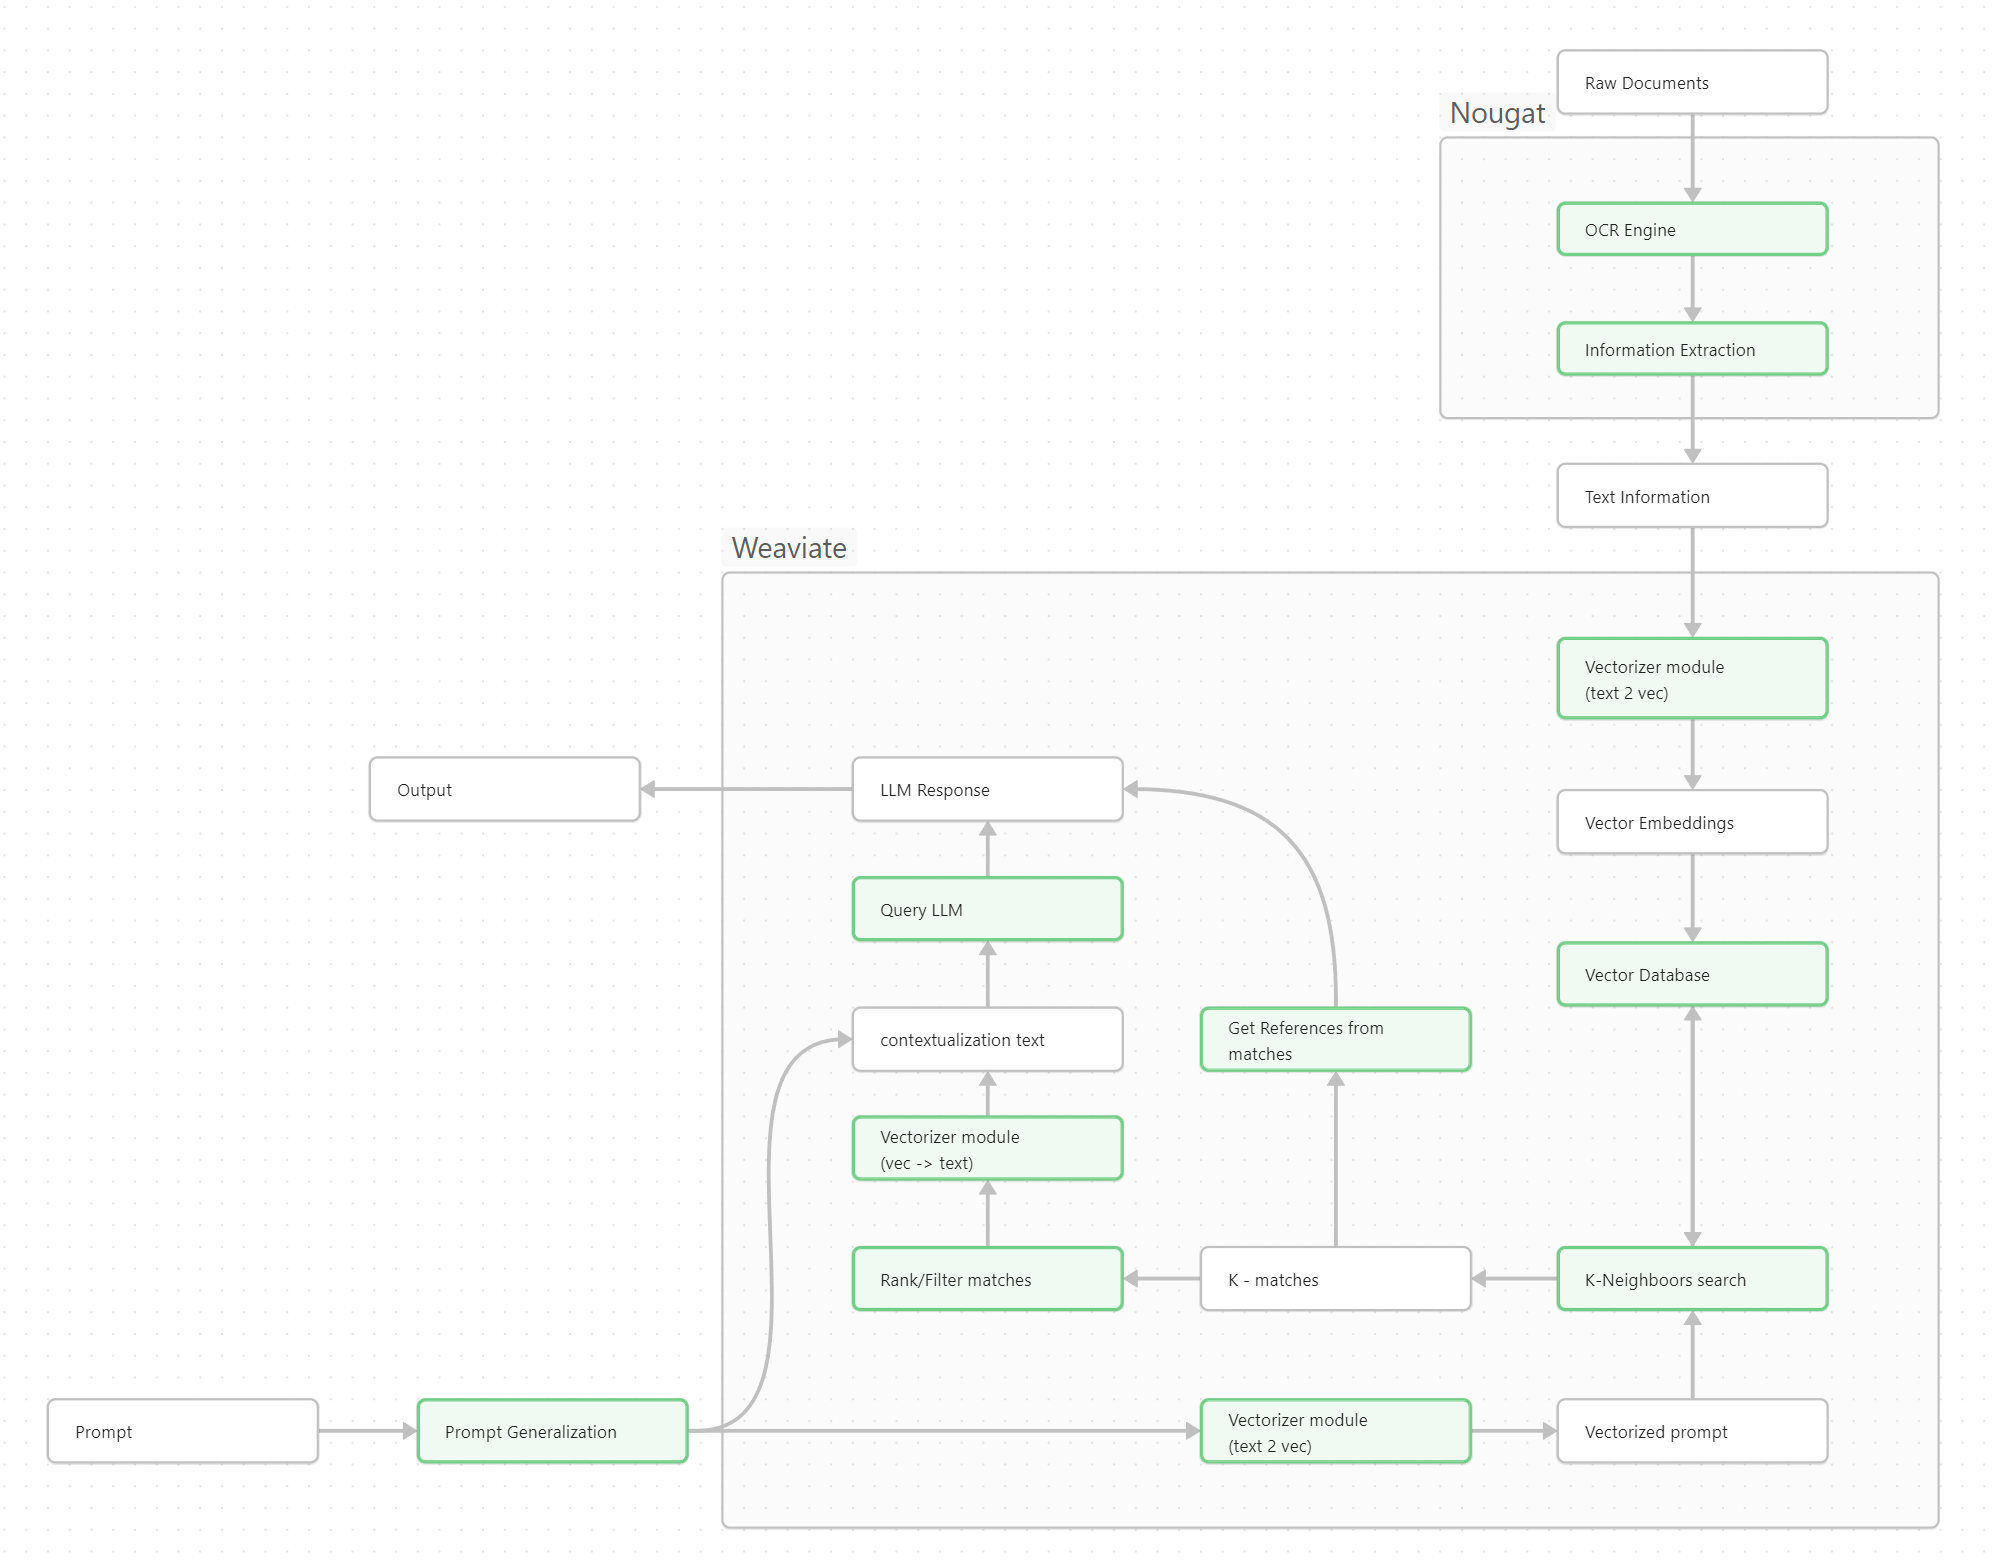
\includegraphics[width=1\linewidth]{Figures/graph_methods.png}
    \caption{Diagram of the project}
    \label{fig:methodology}
\end{figure}

\section{Optical Character Recognition Engines}
\label{sec:ocr}
Most documents in this thesis were digital-born PDFs, where text could be directly extracted with the \texttt{pdfreader} library. To ensure universal applicability of the RAG pipeline, an OCR fallback was included for cases where text was not embedded. 

OCR converts scanned PDFs or images into machine-readable text through preprocessing, segmentation, and recognition. Modern engines combine feature extraction, template matching, and contextual analysis with machine learning. Widely used options include Nougat \cite{blecher2023nougatneuralopticalunderstanding}, which preserves structure and outputs Markdown; Tesseract, an open-source tool supporting over 100 languages; and Google Vision API, a cloud-based service using deep neural networks for high accuracy.

In this thesis, Nougat is used as it is open-source and outputs Markdown, the preferred format for integration with large language models.

\section{Designing the Retrieval-Oriented Weaviate Schema in Edoclink}

The first methodological step was the definition of a semantic data layer using Weaviate, integrated into the Edoclink platform. The goal was to capture the organizational logic of business documents—workflows, stages, entities, folders, and files—within a structure that supports semantic search and generative reasoning. To this end, six core classes were defined (Fluxo, Etapa, Entidade, Pasta, Ficheiro, Metadados), reflecting Edoclink’s information model. These were initially connected through cross-references, ensuring that workflows could be linked to their stages, entities to their folders, and files to their associated metadata.

\begin{figure}[h!]
    \centering
    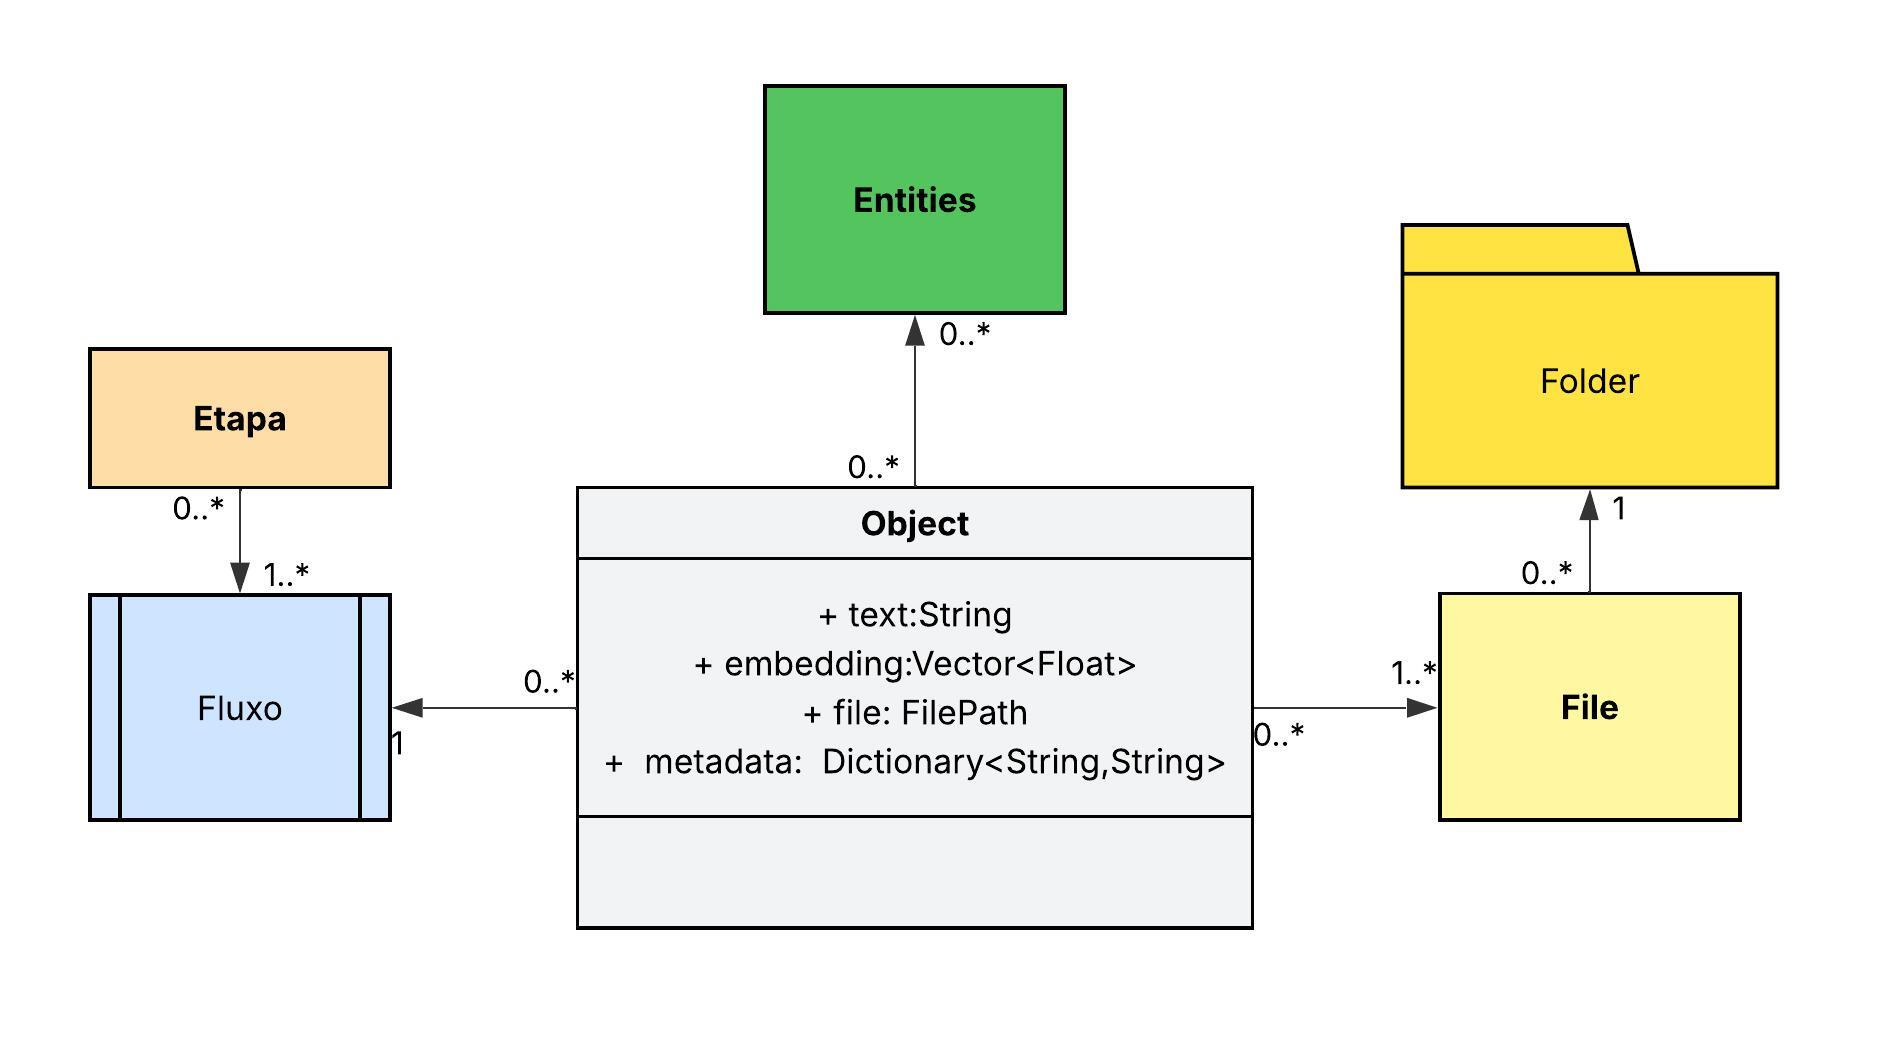
\includegraphics[width=1\linewidth]{Images/Classe UML.jpeg}
    \caption{Abstract UML representation of the schema structure, showing the relationships between objects, entities, folders, files, stages, and workflows in the Edoclink platform.}
    \label{fig:weaviate_class}
\end{figure}

As the research progressed, the schema was refined by embedding \textit{entities}, \textit{file paths}, and \textit{metadata} directly into the object representation. This ensured that objects became self-contained, enabling consistent deletion cascades and reducing reliance on cross-reference traversal for retrieval. The UML diagram in Figure~\ref{fig:weaviate_class} illustrates this abstract model, which was investigated as a candidate for efficient implementation. In practice, the real deployment within Edoclink is more complex, but this abstraction served as a foundation for evaluating design choices and guiding the development of scalable semantic retrieval. The results presented here should therefore be interpreted as a conceptual example rather than a one-to-one description of the production system.

Weaviate natively supports multi-tenancy, and this functionality is employed in Edoclink to store independent datasets under a shared schema, with each instance exposed through web hooks. While not a methodological focus of this work, this results in a decentralized-like architecture, as data is distributed across multiple instances. This design increases the complexity of retrieval, since agents must identify and query the appropriate web hooks when traversing datasets.  

In summary, this section has focused on the database perspective: defining the schema, refining it through embedded fields, and placing it in the context of multi-tenant storage. The next section shifts attention to Agentic AI, where the challenge is not schema design but orchestrating retrieval with agents. This transition reflects the broader research landscape, where developments such as Weaviate’s Query Agent \cite{weaviate} exemplify the move toward automated reasoning layers capable of multi-step retrieval and problem solving.

.


\section{Information extraction and Structuring}
Research will focus on evaluating multimodal models for their ability to capture both textual content and document structure. Models to be studied include:
\begin{itemize}
    \item \textbf{PrimaLayout}: Identifying and classifying regions such as text, tables, and images.
    \item \textbf{PubLayNet}: Segmenting documents into logical blocks.
    \item \textbf{Nougat}: An OCR engine that converts documents into markdown, preserving the hierarchy of chapters, sections, and subsections.
    
\end{itemize}
Testing and integrating the best model to extract and preserve document structure will be studied. Aiming for the structuring of the extracted content for efficient storage and retrieval.
\section{Vector Creation and Storage}
Research with the focus on optimizing the process of generating and storing document embeddings to ensure accurate and fast retrieval. For example finding what embedding models provide the best performance for retrieval, or how can embeddings be stored and queried efficiently at scale.
Tools such as Weaviate will be used to generate vector embeddings. And store in an optimal vector database for retrieval even at scale.

\section{Prompt Engineering}
Integrate a light \ac{LLM} to run locally and serve as the interface for retrieving information from documents, with their embeddings stored in the vector database. Implement techniques to ensure that the user's prompt becomes more consistent before reaching the retrieval stage. Techniques to be investigated include dynamic query refinement, which involves automatically enriching the user prompt by adding missing context, such as prior interactions or user-specific information. Another technique is follow-up questioning, where insufficient context in the user prompt is detected, and clarifying questions are asked to refine the query and provide better retrieval context. For example:
\begin{itemize}
    \item The retrieved documents span multiple categories. Are you specifically interested in category A or category B?
    \item Would like the retrieved documents to focus on a specific time frame or region?
\end{itemize}

\section{Access Control and Security}
Investigate methodologies for access management and stored information security in the context of retrieval systems. Researching encryption and secure storage techniques for embeddings and documents. Study methods to implement user-based access restrictions to ensure privacy and compliance with organizational policies.
Then implement access control mechanisms to restrict users to authorized information. Integrate access management features to make users restriction to information dynamic.

\section{Decentralized Database}
For easier interoperability and integration, the storage for embeddings, generated and document metadata. Which are created from the pre-processing \ac{RAG} pipeline. A type of semantic database is necessary, to enhance semantic search through the internet security. For this a simple server implementation awating for semantic search requests will be implemented.

\section{Semantic Search}
With the use of embedding models. We process the prompt with an llm, for generalizing the prompt for a better search query. Then the embedding of the processed query is generated using the same embedding model used for processing the documents. Then a vector search is done to the vector database. Which finds the most relevant chunks. THe chunks are indexed to the document. The best documents are indexed.
\chapter{Planning}

To achieve the goals outlined above, including chapter \ref{chapter:Planned Results}, the project will be divided into distinct phases \ref{fig:planning}. Each phase will focus on specific milestones to ensure the timely and systematic development of the solution.

\begin{figure}[H]
    \centering
    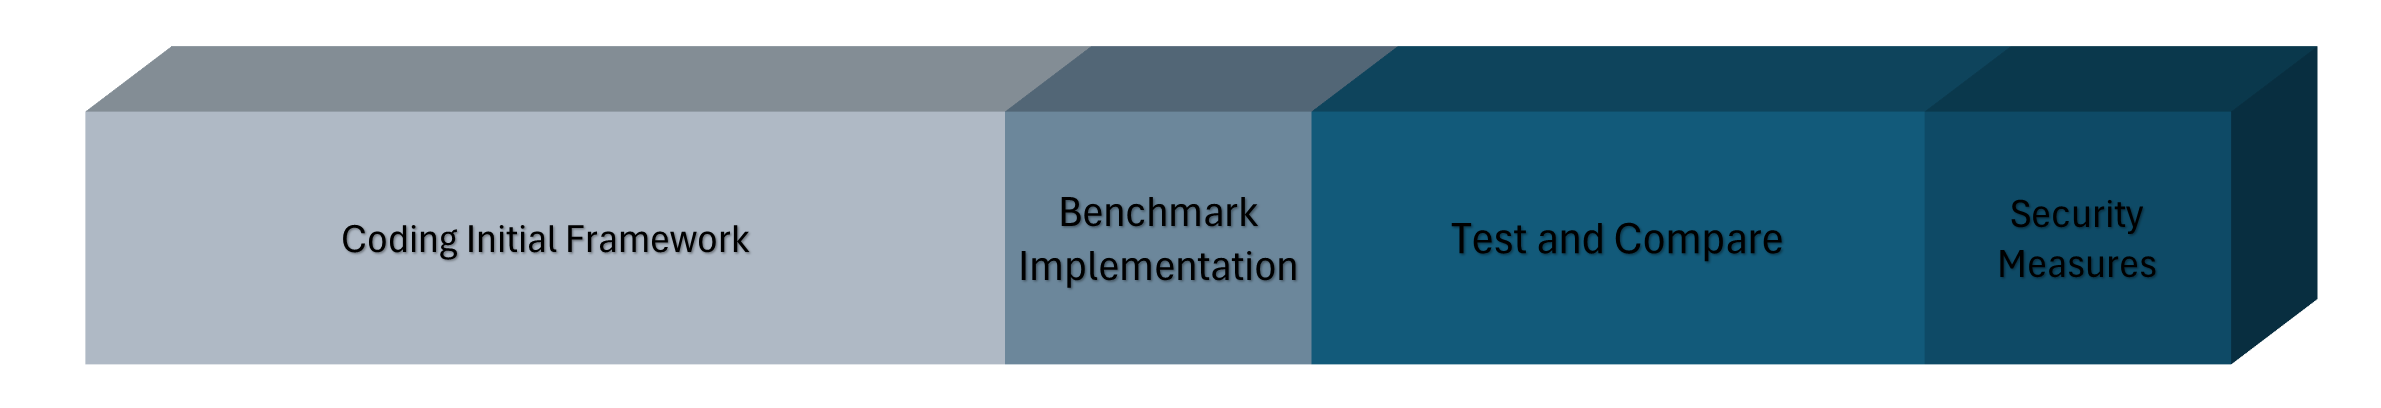
\includegraphics[width=1\linewidth]{Images/planning.png}
    \caption{Simplified Planned Workflow}
    \label{fig:planning}
\end{figure}
\section{Until Now - Initial Research and Pre-processing of Information}
Research has been conducted on \acr{RAG}, \ac{LLM}, and \ac{VD}. Tools like Weaviate have been identified to facilitate the integration of \acr{RAG} and \ac{VD}. By creating collections that combine these techniques, various approaches can be tested and evaluated. Additionally, lightweight \ac{LLM}s such as Llama3.2, which can run fully locally, have been explored. However, considering the rapid advancements in this field, newer lightweight \ac{LLM}s with improved integration capabilities may become available in the future.

A preprocessing pipeline has been developed to extract text from documents while preserving their structure. Several OCR engines, including Google Vision, Tesseract, and Nougat, have been tested. Pre-trained layout models such as PrimaLayout and PubLayNet have also been evaluated. A script was implemented to extract text from PDFs by converting them to PNG format, enabling text extraction using Nougat \cite{blecher2023nougatneuralopticalunderstanding}.

\section{By Month 3 - Initial Framework}

The initial framework will involve creating a collection using Weaviate. Documents will be stored as vector embeddings, enabling vector search techniques such as semantic search and question-answer extraction. This collection will serve as the foundation for testing and experimentation.

\section{By Month 4 - Dataset Creation / Benchmark Implementation}
\label{sec:datasetcreation}
A dedicated dataset will be developed to ensure consistent testing across different techniques for document storage and extraction. AS stated in subsection \ref{subsec:externalbenchmark}, if a recognized external benchmark dataset  for testing vector databases is identified, it will be adopted. Otherwise, a custom dataset will be created with sufficient variety and scale to validate the system, as explained above in chapter \ref{chapter:Planned Results}.

\section{By Month 6 - Testing / Comparative Analysis}

The testing phase will focus on evaluating various techniques for document storage and extraction. \ac{LLM}s will be integrated during this process, as they may enhance certain methodologies. Inspired by prior research such as \cite{densepassageretrievalopendomainkarpukhin2020}, this project aims to achieve improved outcomes using modern, larger-scale models with better training.

Once testing is completed, the best results will be documented as a comparative analysis. Then an \ac{LLM} will be integrated to summarize the output, enabling a concise presentation of the findings.

\section{By Month 7 - Security Measures}

The program will be enhanced with robust security features to ensure controlled access to information. User roles will be defined, including standard users and administrators, where administrators will have the authority to manage access of different users to various types of documents. The program will only be accessible through authenticated user or admin accounts.

Documents will be categorized with tags such as recruitment, human resources, finances, or treasury. Access permissions will be assigned based on user roles, ensuring that each user only has access to the documents relevant to their responsibilities.

An Access Control List (ACL) will be implemented to enforce these restrictions on documents indexed in the \ac{VD}. Additionally, encryption mechanisms will be explored to protect sensitive information further. These security enhancements will be developed in collaboration with LinkConsulting, a company specializing in AI and information storage solutions like EdockLink, with proven expertise in addressing corporate software security requirements.



